%
% db-paretoverteilung.tex -- Datenblatt der Pareto-Verteilung
%
% (c) 2015 Prof Dr Andreas Mueller, Hochschule Rapperswil
%
\subsection{Steckbrief}
\begin{center}
\renewcommand{\arraystretch}{2}
\begin{tabular}{|l|l|}
\hline
Name&Potenzverteilung, Pareto-Verteilung\\
\hline
Dichtefunktion&
\begin{minipage}{3.7in}
\vskip5pt
$\displaystyle
\begin{cases}
\frac{\alpha-1}{x_{\min}}\biggl(\frac{x}{x_{\text{min}}}\biggr)^{-\alpha}&\qquad x>x_{\text{min}}\\
0&\qquad\text{sonst}
\end{cases}
$
\end{minipage}
\\[15pt]
Verteilungsfunktion&
\begin{minipage}{3.7in}
\vskip3pt
$\displaystyle
\begin{cases}
1-\biggl(\frac{x}{x_{\text{min}}}\biggr)^{1-\alpha}&\qquad x>x_{\text{min}}\\
0&\qquad\text{sonst}
\end{cases} $
\end{minipage}
\\
Erwartungswert&$\displaystyle\frac{\alpha-1}{\alpha-2}x_{\text{min}}$,
undefiniert für $\alpha\le 2$\\
Varianz&$\displaystyle
\biggl(
\frac{\alpha-1}{\alpha -3}-\biggl(\frac{\alpha-1}{\alpha-2}\biggr)^2
\biggr)x_{\text{min}}^2$, undefiniert für $\alpha \le 3$\\
$P(|X-E(X)|>\varepsilon)$&$\displaystyle $ \\
Median&$2^{\frac1{\alpha-1}}x_{\text{min}}$\\
\hline
Anwendungen&\begin{minipage}{3.7in}%
\vskip5pt
\strut
$\bullet$ Häufkeitsverteilung für skaleninvariante Prozesse\\
$\bullet$ Einkommensverteilung\\
$\bullet$ Grösse und Häufigkeit von Mondkratern\\
$\bullet$ Verkaufszahlen von Büchern\\
$\bullet$ Einwohnerzahlen von Städten
\strut
\end{minipage}\\[28pt]
\hline
\end{tabular}
\end{center}

\subsection{Wahrscheinlichkeitsdichte}
Wahrscheinlichkeitsdichte einer Potenzverteilung mit $\alpha=2.5$,
diese Verteilung hat keine Varianz:
\begin{center}
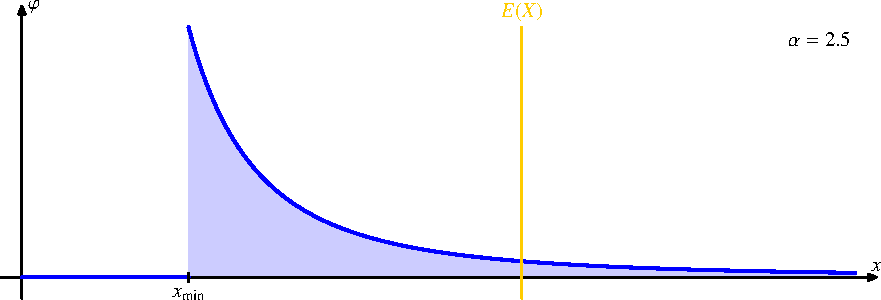
\includegraphics{images/power-2.pdf}
\end{center}

Wahrscheinlichkeitsdichte einer Potenzverteilung mit $\alpha=3.5$:
\begin{center}
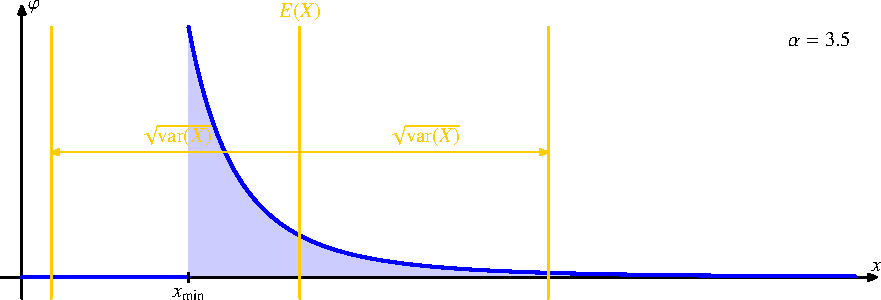
\includegraphics{images/power-3.pdf}
\end{center}

\subsection{80/20-Regeln}
Potenzgesetze geben Anlass zu 80/20-Regeln.
Wir bezeichnen die Wahrscheinlichkeit des Auftretens von Werten $x>0$ 
mit $P(x)=1-F(x)$ und den Anteil des Erwartungswertes dieser Wert
am gesamten Erwartungswert  mit
\[
W(x)=\frac{\int_x^\infty \xi\varphi(\xi)\,d\xi}{\int_{x_{\text{min}}}^\infty \xi\varphi(\xi)\,d\xi}.
\]
Man kann $W(x)$ als den Anteil des ``Wertes'' interpretieren,
den die Werte oberhalb von $x$ beisteuern.
Es ist klar, dass $P(x)=1$ auch bedeutet, $W(x)=1$: 100\% der Werte
tragen 100\% des Wertes bei.
Die Definitionen besagen, dass für beliebiges $x$ der obere $P(x)$-Anteil
der Werte den Anteil $W(x)$ des gesamten Wertes beitragen.
Es gilt
\[
W(x)= P(x)^{\frac{\alpha-2}{\alpha-1}}.
\]
Kurven $(P(x),W(x))$ für verschiedene Werte von $\alpha$:
\begin{center}
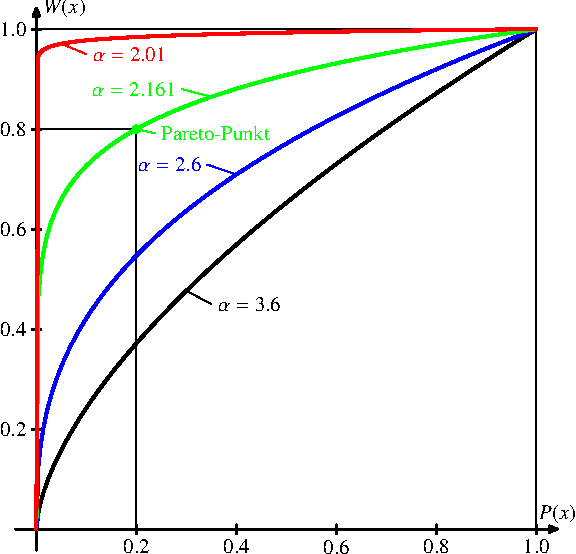
\includegraphics{images/power-4.pdf}
\end{center}

